Dieser Teilerfolg soll nun auch auf zwei Dimensionen, also ein Bild angewendet werden.
Dafür wird ein etwas verschwommenes Dreieck, wie abgebildet links in \ref{deconvolve:example}, als Versuchsabbildung verwendet.
Die Grösse beträgt 9600x9600 Pixel, analog den 9600 Samples der obigen Funktion.
Vorteil diese Bildes ist, dass es Zeilen- und Spaltenweise genau gleich wie das 1D-Signal behandelt werden kann.
\begin{figure}[h]
\centering
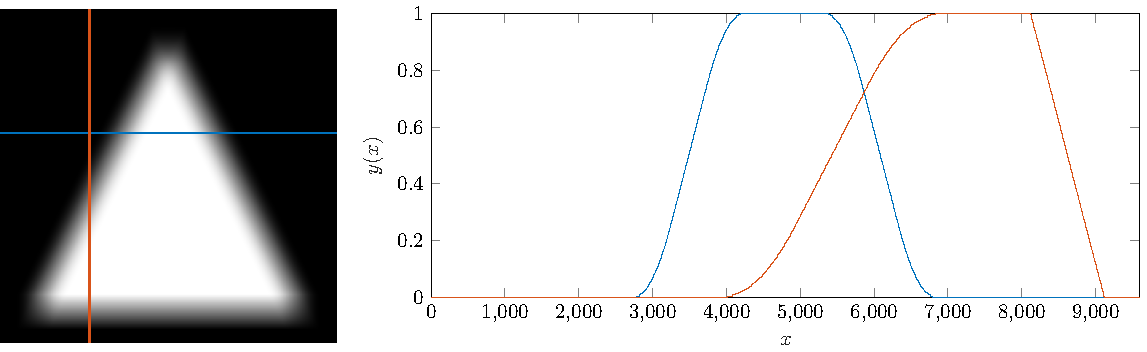
\includegraphics[width=0.9\textwidth]{./papers/deconvolve/pictures/dreieck.pdf}
\caption{Beispielbild\label{deconvolve:example}}
\end{figure}

Die Parameter $m$ und $\alpha$, die vorher für jedes Level einzeln bestimmt wurden, bleiben erhalten.
Die Funktion aus \eqref{deconvolve:funktion} wird also auf alle Level gleich wie oben ausgeführt.
Dies geschieht einmal Zeilen- und Spaltenweise.
Insgesamt wird also 19200 mal eine Analyse mit der diskreten Wavelet-Transformation durchgeführt.
Danach wird das arithmetische Mittel der beiden korrigierten Bilder genommen
$$f_\text{sharp}(x,y)=\frac{f_\text{rows}(x,y)+f_\text{cols}(x,y)}{2}.$$
$f_\text{sharp}$ bezeichnet hierbei das Endergebnis, $f_\text{rows}(x,y)$ und $f_\text{cols}(x,y)$ sind die Zeilen-, bzw. die Spaltenweise \glqq geschärften\grqq{} Varianten des ursprünglichen Bildes.
Abbildung \ref{deconvolve:ergebnis} zeigt das daraus resultierende Ergebnis.
\begin{figure}[h]
\centering
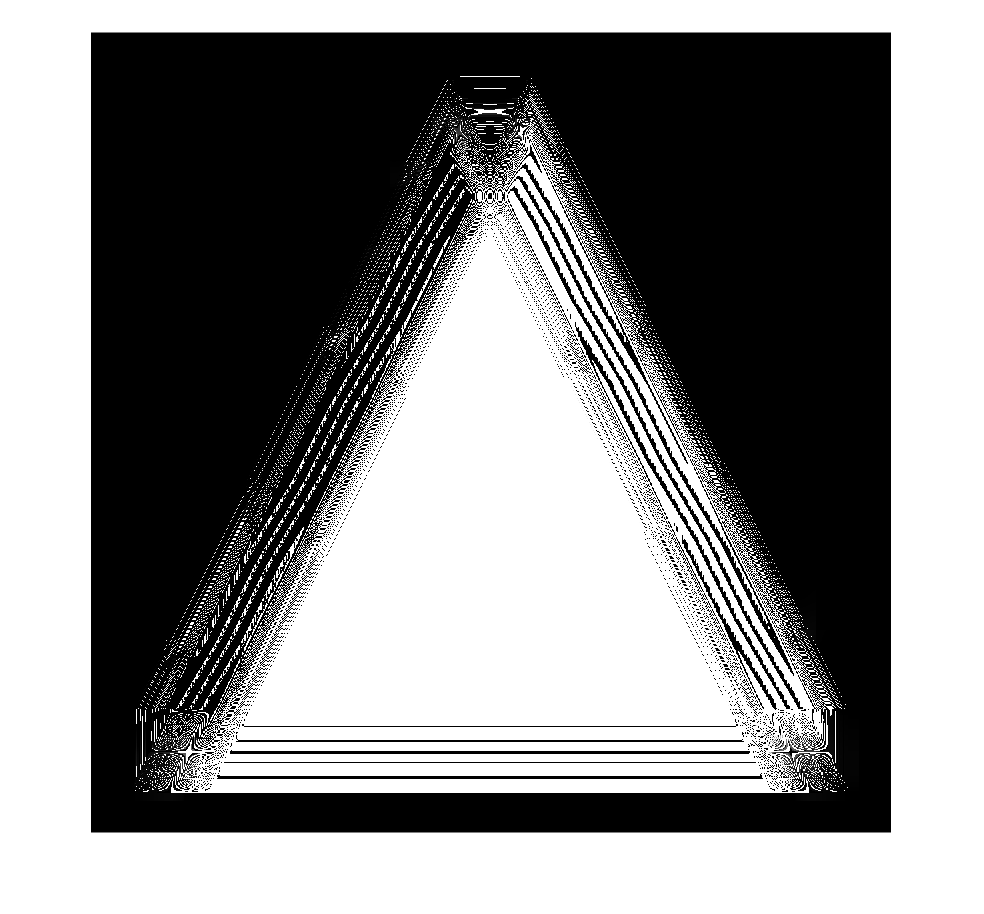
\includegraphics[width=0.7\textwidth]{./papers/deconvolve/pictures/dreieck_sharp.png}
\caption{Ergebnis\label{deconvolve:ergebnis}}
\end{figure}
 
Eine Verbesserung ist nicht zu erkennen. Wo vorher der Rand verschwommen war, sind jetzt einfach starke Schwingungen aufgetreten.